\SourcePage{GELFAND-P000469}{unlabelled}
\Incomplete{GELFAND-P000469}{top-cancelled}{A crossed-out mark before the first line with a short stroke to its right. The reading is unresolved.}
\end{GelfandAdjacentEvidence}
\begin{GelfandAdjacentEvidence}{GELFAND-P000469}{2}

In fact
\SourceFigure{GELFAND-P000469}{inclusion-bracket}{The line under the inclusion turns up at both ends.\par\smallskip\centering
\begingroup\color{black}\GelfandFitDiagram{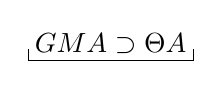
\begin{tikzpicture}
\node[inner sep=2.2pt] (inclusion) at (0,0) {$GMA\supset\Theta A$};
\draw (inclusion.south west) ++(0,4pt) -- (inclusion.south west) -- (inclusion.south east) -- ++(0,4pt);
\end{tikzpicture}}\endgroup}
\end{GelfandAdjacentEvidence}
\begin{GelfandAdjacentEvidence}{GELFAND-P000469}{3}


\uline{Mark the vertex \mbox{$0$}} — the identity of the group $GMA$.

\uuline{\mbox{$SA$}} — the corresponding simplicial scheme.

(Historical remark: Volodin used $SA$ to define the functors $K_{\mathbb C}^{n}$)
\par in essence
\Unclear{GELFAND-P000469}{top-functor-index}{The subscript reads $\mathbb C$, with an extra stroke inside the letter.}
\end{GelfandAdjacentEvidence}
\begin{GelfandAdjacentEvidence}{GELFAND-P000469}{4}


{\centering\rule{2.7em}{.4pt}\quad\textperiodcentered\quad\rule{3.1em}{.4pt}\par}
Suppose the ring $A$ has a unit. Then put.
\[
K_nA=\pi_{n-1}SA,\qquad n\geqslant1.
\]
For $n\geqslant2$ there is a group structure, commutative for $n\geqslant3$.

\uline{Another def. of the group structure (commutative).}

\uline{Whitehead's lemma}

Consider the spheroid $s\colon Z^n\longrightarrow SA$.
The group of permutations acts on $SA$ $f\colon N\longrightarrow N$.
We obtain a new spheroid $s^f$:
\SourceFigure{GELFAND-P000469}{spheroid-diagram}{The top arrow is unlabelled.\par\smallskip\centering
\begingroup\color{black}\GelfandFitDiagram{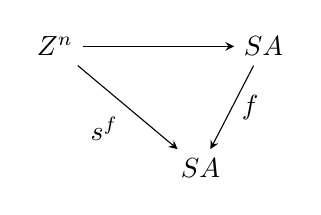
\begin{tikzpicture}[>=stealth]
\node (sphere) at (0,0) {$Z^n$};
\node (top) at (2.65,0) {$SA$};
\node (bottom) at (1.85,-1.55) {$SA$};
\draw[->] (sphere) -- (top);
\draw[->] (sphere) -- node[below left] {$s^f$} (bottom);
\draw[->] (top) -- node[right] {$f$} (bottom);
\end{tikzpicture}}\endgroup}
\end{GelfandAdjacentEvidence}
\begin{GelfandAdjacentEvidence}{GELFAND-P000469}{5}


They are always homotopic.

\uline{Idea of the proof:}

$\operatorname{Im}s\subset M_kA$.
\[
s=\left(\begin{array}{c|c}sz&0\\\hline 0&0\end{array}\right).
\]
Everything reduces to the case
\[
s^f=\left(\begin{array}{c|c}0&0\\\hline 0&sz\end{array}\right).
\]
\Unclear{GELFAND-P000469}{middle-block-argument}{The final sign in $sz$ has a cross-stroke and is provisionally set as a lowercase letter. Both matrices have two dividing rules.}
\end{GelfandAdjacentEvidence}
\begin{GelfandAdjacentEvidence}{GELFAND-P000469}{6}


($f$ of a special form: $fi=i+k$, we adjust it at $\infty$).

\[
\begin{pmatrix}a&0\\0&0\end{pmatrix}\quad
\begin{pmatrix}a&a\\0&0\end{pmatrix}\quad
\begin{pmatrix}0&a\\-1&0\end{pmatrix}\quad
\begin{pmatrix}0&0\\-1&a\end{pmatrix}\quad
\begin{pmatrix}0&0\\0&a\end{pmatrix}
\]
\Unclear{GELFAND-P000469}{five-spheroids}{The upper left zero in the third matrix is heavily retraced.}
\end{GelfandAdjacentEvidence}
\begin{GelfandAdjacentEvidence}{GELFAND-P000469}{7}

These are 5 spheroids. This is a homotopy. Each 2 neighbours are elementarily homotopic:

\[
s_1,s_2\colon S'\longrightarrow S'
\]
are called elem. homotopic if $\forall$ simplices $X\subset S$, $s_1X\cup s_2X$
is a simplex in $S'$.
\Unclear{GELFAND-P000469}{homotopy-domain}{A short stroke is visible above the first $S$. The next line has $X\subset S$ without a prime.}
\end{GelfandAdjacentEvidence}
\begin{GelfandAdjacentEvidence}{GELFAND-P000469}{8}


Let all $a$ lie in one simplex $X$.
Then $\begin{pmatrix}a&0\\0&0\end{pmatrix}$ and
$\begin{pmatrix}a&a\\0&0\end{pmatrix}$ lie in one simplex.

Let $a_0^{-1}\in X$. Multiply by $a_0$. Then they become upper triang.
If all $a$ are upper triangular, then all 5 matrices lie in one simplex.

{\centering\rule{3em}{.4pt}\quad\textperiodcentered\quad\rule{3.5em}{.4pt}\par}
\uline{The commutative group structure on \mbox{$K_nA$}.}
\[
MA\times MA\xrightarrow{\oplus}MA
\]
\[
\begin{array}{@{}ll|l@{}}
fi=2i & f,g\colon\mathbb N\longrightarrow\mathbb N & \text{noncommut., nonassoc., with no}\\
gi=2i+1 & a\oplus b=a^f+b^g & \text{identity elem.}
\end{array}
\]
\SourceFigure{GELFAND-P000469}{group-operation-margin}{A vertical rule separates the note about the operation.}
\end{GelfandAdjacentEvidence}
\begin{GelfandAdjacentEvidence}{GELFAND-P000469}{9}


\Unclear{GELFAND-P000469}{margin-left-bottom}{Outside the left edge of the text are a slanting stroke and a mark resembling a closing parenthesis. Their purpose is unresolved.}
\end{GelfandAdjacentEvidence}



\Needspace{7\baselineskip}
\begin{GelfandAdjacentEvidence}{GELFAND-P000470}{1}
